\documentclass[11pt]{article}
\usepackage[utf8]{inputenc}
\usepackage{amsmath, amssymb}
\usepackage{geometry}
\geometry{a4paper, margin=1in}
\usepackage{tikz}
\usepackage{enumitem}
\usepackage{hyperref}

\title{Technical Summary: Optimal Deterministic Massively Parallel Connectivity on Forests}
\author{}
\date{}

\begin{document}

\maketitle

\section{Problem and Contribution}

\subsection{Problem}
The paper tackles the \textbf{connected components} problem in the low-space Massively Parallel Computation (MPC) model on \textbf{forests} (graphs without cycles). Given a forest with \(n\) nodes (\(n\) is the total number of vertices, e.g., dots in the graph) and \(m\) edges (\(m\) is the number of connections, where \(m = n - k\) and \(k\) is the number of trees), the objective is to assign each node a label identifying its component, typically the maximum node ID in its tree. This fundamental graph problem has applications in network analysis, clustering, and data partitioning. The challenge lies in solving it efficiently in a parallel setting where each machine has limited memory (\(S = n^\delta\), where \(S\) is local memory per machine and \(\delta\), \(0 < \delta < 1\), is a memory exponent balancing memory and parallelism) and total memory is \(O(n + m)\).

\subsection{Contribution}
The main contribution is a \textbf{deterministic algorithm} that solves connected components on forests in \(O(\log D)\) rounds, where \(D\) is the maximum diameter of any tree (the longest path between any two nodes in a single tree, measured in steps). Key aspects include:
\begin{itemize}
    \item \textbf{Optimality}: Matches a conjectured lower bound (1 vs. 2 cycles conjecture).
    \item \textbf{Diameter-Driven}: Complexity depends on \(D\), not \(n\), unlike prior \(O(\log n)\) methods.
    \item \textbf{Generalizability}: Extends to rooting forests and solving Locally Checkable Labeling (LCL) problems.
\end{itemize}
This is a significant advance over deterministic \(O(\log n)\) MPC algorithms, offering faster runtime for forests with small \(D\).

\section{Algorithmic Description}

\subsection{Core Idea}
The algorithm iteratively compresses the forest into a smaller graph, solves the problem on the compressed version, and decompresses to propagate the solution. It leverages the \textbf{MAX-ID problem}: each node learns the maximum ID in its tree. The process reduces the graph’s diameter in \(O(\log D)\) rounds while adhering to MPC memory constraints.

\subsection{Inputs and Outputs}
\begin{itemize}
    \item \textbf{Input}: A forest \(G = (V, E)\) with \(n = |V|\), \(m = |E|\), and unique node IDs (\(id(v)\) is the unique identifier of node \(v\)).
    \item \textbf{Output}: Each node \(v\) outputs \(\max\{id(u) \mid u \in C(v)\}\), where \(C(v)\) is the component (tree) containing \(v\).
    \item \textbf{Model}: \(M = O((n + m) / n^\delta)\) machines (\(M\) is the number of parallel machines), each with \(S = n^\delta\) memory, total \(O(n + m)\).
\end{itemize}

\subsection{High-Level Logic}
\begin{enumerate}
    \item \textbf{Compression Phases}:
        \begin{itemize}
            \item \textit{CompressLightSubTrees}: Merge small subtrees (size \(\leq n^{\delta / 8}\)) into heavy nodes.
            \item \textit{CompressPaths}: Contract paths (degree-2 chains) into single edges.
            \item Repeat \(O(1)\) times until graph size is \(n^{\delta / 2}\).
        \end{itemize}
    \item \textbf{Solve on Small Graph}: Compute max IDs on the compressed graph.
    \item \textbf{Decompression}: Reverse compression, propagating max IDs.
\end{enumerate}

\subsection{Routines and Subroutines}
\begin{itemize}
    \item \textbf{CompressLightSubTrees (Section 4.3)}:  
        Each node \(v\) maintains \(S_v\) (the set of nodes \(v\) knows about in its tree) and a state (Active, Happy, Full, Sad). In \(O(\log D)\) rounds:
        \begin{itemize}
            \item \textit{Probing}: Estimate subtree sizes (\(B_{v \rightarrow u}\), the number of nodes in the subtree from \(v\) toward neighbor \(u\)).
            \item \textit{Exponentiation}: Expand \(S_v\) toward smaller directions, respecting memory.
            \item \textit{Compression}: Happy nodes merge into Full/Sad neighbors.
        \end{itemize}
        \textit{Example}: In 1--2--3--4, 1 compresses into 2 if the subtree of 1 is small (\(B_{2 \rightarrow 1} = 1\)).
    \item \textbf{CompressPaths (Section 4.4)}:  
        Replace paths (e.g., 1--2--3) with edges (1--3), updating max IDs.  
        \textit{Example}: 1--2--3--4 \(\rightarrow\) 1--3--4 \(\rightarrow\) 1--4.
    \item \textbf{Decompression}: Reverse steps to assign max IDs.
\end{itemize}

\subsection{Diagram}
The diagram below shows the compression of 2 ssimple subtrees:
\begin{center}
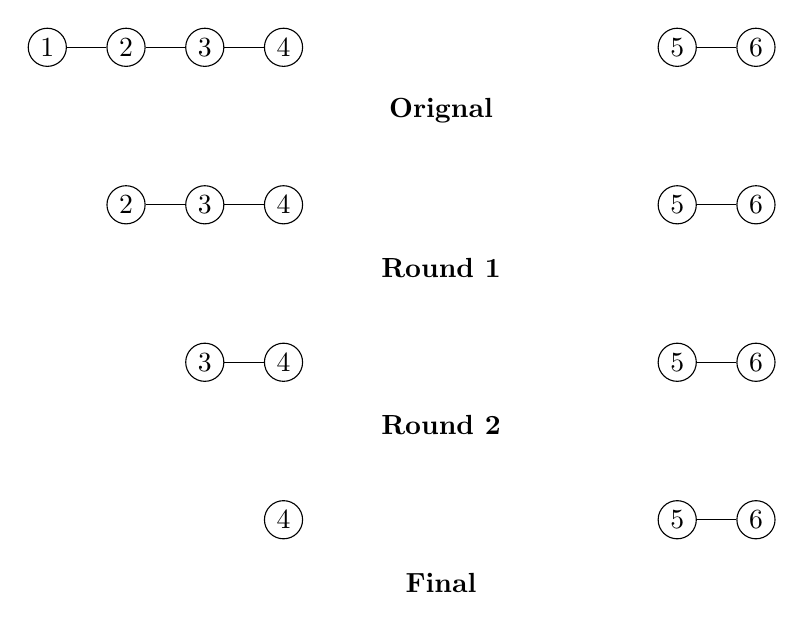
\begin{tikzpicture}
    % Original
    \node[circle, draw, inner sep=2pt] (n1) at (0,0) {1};
    \node[circle, draw, inner sep=2pt] (n2) at (1,0) {2};
    \node[circle, draw, inner sep=2pt] (n3) at (2,0) {3};
    \node[circle, draw, inner sep=2pt] (n4) at (3,0) {4};
    \node[circle, draw, inner sep=2pt] (n5) at (8,0) {5};
    \node[circle, draw, inner sep=2pt] (n6) at (9,0) {6};
    \draw (n1) -- (n2) -- (n3) -- (n4);
    \draw (n5) -- (n6);
    \node at (5, -0.8) {\textbf{Orignal}};

    % Round 1
    \node[circle, draw, inner sep=2pt] (r1n2) at (1,-2) {2};
    \node[circle, draw, inner sep=2pt] (r1n3) at (2,-2) {3};
    \node[circle, draw, inner sep=2pt] (r1n4) at (3,-2) {4};
    \node[circle, draw, inner sep=2pt] (r1n5) at (8,-2) {5};
    \node[circle, draw, inner sep=2pt] (r1n6) at (9,-2) {6};
    \draw (r1n2) -- (r1n3) -- (r1n4);
    \draw (r1n5) -- (r1n6);
    \node at (5, -2.8) {\textbf{Round 1}};

    % Round 2
    \node[circle, draw, inner sep=2pt] (r2n3) at (2,-4) {3};
    \node[circle, draw, inner sep=2pt] (r2n4) at (3,-4) {4};
    \node[circle, draw, inner sep=2pt] (r2n5) at (8,-4) {5};
    \node[circle, draw, inner sep=2pt] (r2n6) at (9,-4) {6};
    \draw (r2n3) -- (r2n4);
    \draw (r2n5) -- (r2n6);
    \node at (5, -4.8)  {\textbf{Round 2}};

    % Round 3
    \node[circle, draw, inner sep=2pt] (r3n4) at (3,-6) {4};
    \node[circle, draw, inner sep=2pt] (r3n5) at (8,-6) {5};
    \node[circle, draw, inner sep=2pt] (r3n6) at (9,-6) {6};
    \draw (r3n5) -- (r3n6);
    \node at (5, -6.8)  {\textbf{Final}};
\end{tikzpicture}
\end{center}




\section{Comparison}

\subsection{Existing Approaches}
\begin{itemize}
    \item \textbf{Randomized MPC}: Achieved \(O(\log n)\) rounds (e.g., Lattanzi et al.) using randomization.
    \item \textbf{Deterministic MPC}: Took \(O(\log n)\) rounds (e.g., Andoni et al.), even on trees.
    \item \textbf{LOCAL Model}: \(O(D)\) rounds, but MPC’s memory limits complicate this.
\end{itemize}

\subsection{Novelty and Improvement}
\begin{itemize}
    \item Deterministic \(O(\log D)\), faster than \(O(\log n)\) when \(D \ll n\).
    \item Exploits forest structure (no cycles) to focus on diameter.
    \item Avoids randomness for reliability.
    \item Matches conjectured lower bound.
\end{itemize}

\section{Data Structures and Techniques}

\subsection{Algorithm Overview}
The method follows a \textbf{compress-solve-decompress} paradigm, designed for efficient parallelization across distributed environments such as those supported by Dask or across multiple machines:

\begin{enumerate}
    \item \textbf{Compress}: Iteratively reduces the forest into a smaller graph using subtree and path compression routines.
    \item \textbf{Solve}: Computes the MAX-ID problem on the reduced graph using centralized computation.
    \item \textbf{Decompress}: Propagates the solution back to the original nodes using stored compression mappings.
\end{enumerate}

\subsection{Core Data Structures}
\begin{itemize}
    \item \textbf{Graph Representation}: Adjacency lists partitioned across machines for scalability.
    \item \textbf{Knowledge Sets (\(S_v\))}: Track discovered nodes, constrained to $O(n^\delta)$ to remain within local memory limits.
    \item \textbf{State Variables}: Each node maintains its status (\texttt{Active, Happy, Full, Sad}) and edge-bound estimates ($B_{v \rightarrow u}$).
    \item \textbf{Aggregation Trees}: Used to manage merges involving high-degree nodes (see Appendix A).
    \item \textbf{Compression Maps}: Record node merges to enable accurate decompression in later stages.
\end{itemize}

\subsection{Compression Techniques}
\textbf{CompressLightSubTrees}: Merges small subtrees (of size $\leq n^{\delta/8}$) into neighboring heavy nodes.

\begin{itemize}
    \item Relies on phased expansion of knowledge sets to estimate subtree sizes.
    \item Nodes transition between states and merge when they satisfy certain conditions (e.g., becoming ``Happy'').
\end{itemize}

\textbf{CompressPaths}: Identifies and collapses paths of degree-2 nodes into single edges.

\begin{itemize}
    \item Efficiently removes long chains to reduce graph diameter.
    \item Updates adjacency structures and prepares the graph for the solve phase.
\end{itemize}

\subsection{Technical Highlights}
\begin{itemize}
    \item \textbf{Balanced Knowledge Propagation}: Employs doubling to grow knowledge sets within memory constraints.
    \item \textbf{Graph Diameter Reduction}: Each compression phase provably reduces the diameter, facilitating faster global communication.
    \item \textbf{Guess-and-Check Techniques}: Unknown parameters like diameter ($D$) are estimated via doubling strategies.
    \item \textbf{Two-Phase Compression}: Separates compression of trees and paths for better structure preservation and efficiency.
\end{itemize}


\section{Implementation Outlook}

\subsection{Potential Technical Challenges}
\begin{enumerate}
    \item \textbf{Memory Management}: Ensuring \(S_v \leq n^\delta\), total \(O(n + m)\). Use sparse representations for sets.
    \item \textbf{Synchronization}: Simulating MPC rounds across two physical machines or using Dask to coordinate distributed workers.
    \item \textbf{Large Input Size}: If \(n \gg 10^6\), a single machine may not suffice. Scale tests to \(10^3\)--\(10^4\) nodes initially.
    \item \textbf{Compression Complexity}: Tracking transformations to enable accurate decompression. Maintain lightweight logs for each step.
    \item \textbf{Numerical Precision}: Since IDs are integers, use 64-bit integers to support large-scale graphs.
\end{enumerate}

\subsection{Implementation Tips}
\begin{itemize}
    \item Use \textbf{Python} with \texttt{NetworkX} for graph handling and \texttt{Dask} for distributed processing.
    \item For parallel execution, either:
        \begin{itemize}
            \item Launch Dask workers on two separate physical machines (with shared configuration), or
            \item Run multiple Dask workers on a single multi-core machine for testing.
        \end{itemize}
    \item Begin testing on forests with \(n = 100\) and \(D = 10\) to validate correctness before scaling.
    \item Keep intermediate compression state for debugging and decompression tracing.
\end{itemize}


\end{document}